% This version of CVPR template is provided by Ming-Ming Cheng.
% Please leave an issue if you found a bug:
% https://github.com/MCG-NKU/CVPR_Template.

\documentclass[final]{cvpr}

\usepackage{times}
\usepackage{epsfig}
\usepackage{graphicx}
\usepackage{amsmath}
\usepackage{amssymb}

% Include other packages here, before hyperref.
\usepackage{csquotes}

% If you comment hyperref and then uncomment it, you should delete
% egpaper.aux before re-running latex.  (Or just hit 'q' on the first latex
% run, let it finish, and you should be clear).
\usepackage[pagebackref=true,breaklinks=true,colorlinks,bookmarks=false]{hyperref}


\def\cvprPaperID{****} % *** Enter the CVPR Paper ID here
\def\confYear{2021}
%\setcounter{page}{4321} % For final version only

\newcommand{\q}[1]{\enquote{#1}}
\newcommand{\Set}[1]{\left\{ #1 \right\}}

\usepackage{amsmath}
\usepackage{amssymb}
\newcommand{\R}{\mathbb{R}}

\begin{document}

%%%%%%%%% TITLE
\title{
	Assignment 4 - Neural Network Recommendation System \\~\\
	\large{Team name: M2 Robo}
}

\author{
	Chan Kwan Yin\\
	3035466978 \\
	Team leader

	\and

	Lee Chun Yin\\
	3035469140\\

	\and

	Chiu Yu Ying\\
	3035477630
}

\maketitle

\clearpage

\section{Background}

Among all collaborative filtering techniques, matrix factorization (MF) become a standard approach to the model-based recommendation. Many research teams have put their efforts on enhancing it to break the accuracy record. 

However, it has several limitations such as the cold-start problem -- how the system provide recommendations to new users, how to recommend when new item is added without feature vector or embedding \cite{FMF}. Also, the use of dot product for recommending popular items will lead to the tendency of recommending popular items to those users without specific user interests. With the use of inner product of User and item feature embeddings, MF limits the capture of the complex relations  of the users and items interactions \cite{NeuralCF}.

In this assignment, we aim to implement the new approach, Neural Collaborative Filtering (NCF), proposed by He team in 2017 \cite{NeuralCF}. They suggested that their design of deep neural network can overcome the limitation of MF.

\section{Neural Collaborative Filtering (NCF) model}

This is the model proposed by He team in 2017 \cite{NeuralCF}. Their proposed model uses a combination of matrix factorization and multi-layer perceptron techniques, and the hidden layers from the two techniques are combined by a fully-connected layer. However, their paper mainly focuses on the prediction of \textit{implicit user feedback}, that is, they are predicting the values of $y_{ui}$ where $y_{ui}=1$ when the obervation (user $u$, item $i$) is observed, and $0$ when the
observation (user $u$, item $i$) is not observed. Thus, at the final stage of their proposed model, the output of the fully-connected layer is passed into a sigmoid function, such that the model only outputs values within $[0, 1]$. 

The problem of predicting implicit feedback is different from the problem we wish to solve in the Netflix dataset, because in the Netflix problem we wish to predict actual ratings from $[1, 5]$.
Nevertheless, we still think that He's paper provides a good starting point - We modify He's model by removing the final sigmoid function and changing the loss functions used directly, such that the neural network solves a regression problem instead of the original binary
classification problem.

The model proposed by He is split into 3 parts - Generalized Matrix Factorization, Multi-Layer Perceptron, and Neural matrix factorization. In fact, the third part is a combination of the previous two parts. For this part of our project, we will follow the same workflow as He and implement the 3 parts separately. 

\begin{figure}[h]
	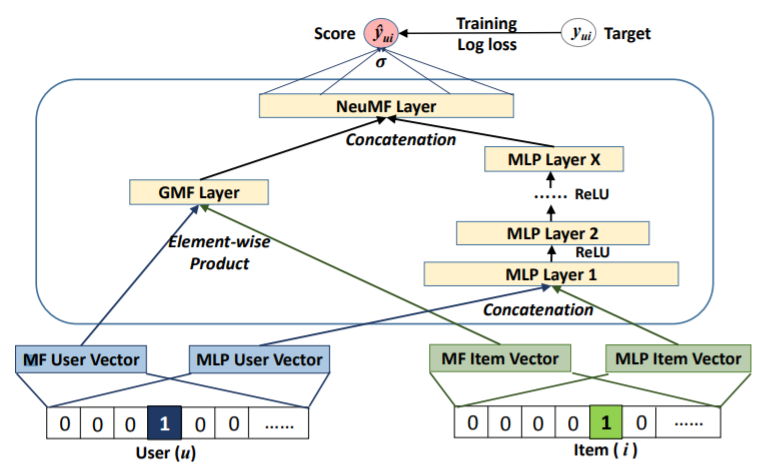
\includegraphics[width=0.5\textwidth]{./NeuCF.PNG}
	\caption{Neural Collaborative Filtering Model Design \cite{NeuralCF}}
\end{figure}

\

This model adopts the multi-layer perceptron (MLP) to model the user-item interaction $y_{ij}$.
We take two vectors from user and item respectively in the input layer and then they will be embedded to pass the neural collaborative filtering (neural CF) layers. In our neural CF layers, we first do matrix multiplication. The product then passes into the rectified linear unit (ReLU) and next passes through an activation function $f1(x)$.

% \subsubsection{Model - Input Layer}

This model takes two sparse feature vectors from representation of users and items respectively. 

\begin{itemize}
	\item User vector:$v_i$ with m users 
	\item Item vector:$v_j$ with n items.

\end{itemize}
The identity of users and item will be transformed to a binarized vector with one-hot encoding. 

With such generic feature representation, the model can handle various modelling types such as content-based and neighbor-based. The limitation of the cold-start problem can be solved by using the content features to represent users and items.

% \subsubsection{Model - Embedding Layer}

After the input layer, the next is the embedding layer. It is fully connected to project the sparse vector representations ($v_i$ and $v_j$) for users and items in the input layer into dense vectors.It can also be seen as the latent vector matrix, $P$ for users and $Q$ for items, in the context of latent factor model.


% \subsubsection{Model - Neural Collaborative Filtering Layer}
The obtained latent vectors from the embedding layers will then be fed into the the neural CF layers,and be mapped to predicted probability scores by mapping fuction $\phi_X$. Those layers will get the complex user-item relations from the vectors.

% \subsubsection{Model - Output Layer}

The final output layer produces a predicted score $\hat{y_{ij}}$, which is the predicted user-items interactions of $y_{ij}$ through the mapping function $\phi_{output}$.



% \subsubsection{Model - Formula}
\bigskip
\textbf{ The formula of the NCF is as follow:}
$$\hat{y_{ij}} = f(P^T v_i Q^T v_j|P,Q,\Theta_f)$$

The variables with m users and n items are denoting as:
\begin{itemize}
    \item $P \in \R^{(m \times K)}$ latent factor matrix for users from embedding layer.
    \item $Q \in \R ^{(n \times K)}$ latent factor matrix for items from embedding layer.
    \item $f$ interaction function.    
    \item $\Theta_{f}$ model parameters of the interaction function $f$
\end{itemize}

\bigskip
\textbf{ For interaction function $f$, it can be formulated:}
$$f(P^T v_i, Q^T v_j) = \phi_{output}(\phi_X(...\phi_2(\phi_1(P^T v_i, Q^T v_j))...))$$

The mapping functions are as follow:
\begin{itemize}
    \item $\phi_{output}$: the mapping function for output layer
    \item $\phi_x$ the mapping function for the xth neural CF layer. X is the number of the layers
\end{itemize}

% \subsection{Neural Network Model}


\section{Technical Details}
The training data set provided by Netflix consists of more than 100 million ratings with 17770 movies and 480189 users.
% Such a huge data set would consume a significant amount of training time and memory
% ($O(m^2 n)$, since a correlation matrix between users is to be constructed),
% which is not possible for our hardware available.
% Therefore, only a subset of data is used for evaluation.
% To be specific, only first $10000$ movies and first $1000$ users that appear in the data set are considered.

\subsection{Data preprocessing}
The movies are loaded into a list with columns of Movie ID, User ID and Rating. Then, it will be fed into the test loader with batch size.


% Approximately $80\%$ data are then reformatted into a rating matrix $R \in \mathbb R^{m \times n}$ for training,
% where $r_{ij}$ is the rating of user $i$ on movie $j$;
% the rest are retained for performance evaluation.
% The missing data are being skipped in our model.


%In general, our algorithm runs through all rows for $\epsilon+1$ times
% where $\epsilon$ is the number of epochs of gradient descent.
% The model involves 5 parameters,
% namely $\mu \in \mathbb R, \mathbf b \in \mathbb R^m, \mathbf c \in \mathbb R^n, P \in \mathbb R^{mk}, Q \in \mathbb R^{nk}$.
% The blocking term is $nk$, so this model is scalable to the full dataset given that $nk$ is not beyond memory limit.
% We have not used the full model in this assignment due to time constraints,
% but we will do so in the final report.

\subsection{Optimization and scheduler}
We select Adadelta as our optimizer. 
% To have a better performance on the converge of loss function, we implement a scheduler with step size = 1 and $\gamma$ = 0.7.

To have a better performance on the converge of loss function,we implement a scheduler with different combinations of hyperparameters of scheduler
\subsection{Hyperparameters selection for scheduler}
There are two hyperparameters, namely
\begin{itemize}
    \item step size
    \item $\gamma$
\end{itemize}

\subsubsection{Step size}
tbc

\subsubsection{$\gamma$}
tbc

\subsection{Hyperparameters selection for model}
In this MLP model, there are five hyperparameters to be selected, namely
\begin{itemize}
	\item Learning Rate ($\alpha$)
	\item Regularization ($\lambda$)
	\item Rank of factorization ($k$)
	\item Number of epoch ($x$)
	\item Batch Size ($N$)
% 	\item Log Interval ($t$)
\end{itemize}


\subsubsection{Learning Rate ($\alpha$)}
The learning rate indicates the speed at which the model learns. It controls how much to change the modal to respond the estimate error each time when the model weights are updated.

Rate with too small value may cause a long training time while a large value may allow the modal learning too fast to have less accurate or even not meaningful result.

\subsubsection{Regularization ($\lambda$)}
% Regularization plays a crucial role in preventing the overfitting issue when training model. It aims to reduce the complexity of model to achieve its function. When the regularization parameter is large, the decay in weights during SGD update will be increased and therefore the weights of the hidden units will be negligible (close to zero).

% If it is set to be too large, each change to the parameters are cancelled by the regularization term. If it is set to be too small, overfitting may result.

\subsubsection{Rank of factorization ($k$)}
Intuitively, each rank represents some characteristic of a user or a movie. Users and movies that interact strongly on a rank would be affected.

A large value of $k$ increases the training time, memory consumption and probably the chance of overfitting,
while a low value of $k$ reduces the representativeness of the model and hence reduced accuracy.

\subsubsection{Number of epoch ($x$)}
The number of epochs defines the number of times that the modal will work through the whole training dataset.
Since we already report the training score for each epoch, it is adjusted to a value such that the training score appears to converge negligibly.

% \subsubsection{Log-interval ($t$)}

\subsubsection{Batch size ($N$)}
The batch size defines the number of samples to be passed through before the update of model parameters.

The small batch size usually can give a better performance since the model can start learning with a small subset and have more cycles to improve.

However, the smaller batch size costs the slower learning and hence more training time.

\subsection{Predictive test set score (RMSE)}
The model is evaluated by computing the RMSE between predicted and actual rating values:
$$ \text{RMSE} = \sqrt{\sum_{(i, j) \in E} \frac{{(\hat r_{ij} - r_{ij})}^2}{\left| E \right|}} $$
where $E$ is the set of retained evaluation data.

\section{Model performance}
The following table exhaustively lists our test results. Train RMSE and Test RMSE refer to the RMSE value calculated for the training dataset and testing dataset respectively.

100,40
Epoch 39, mse = 0.8843765864636746
Test RMSE: 1.0292723480987729

\begin{figure}[h]
	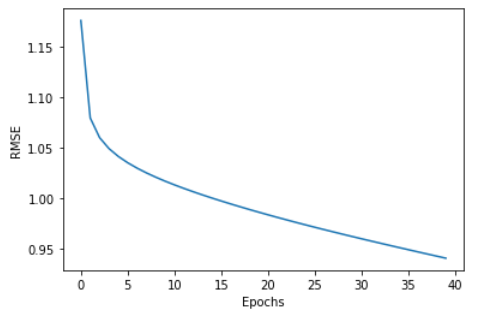
\includegraphics[width=0.5\textwidth]{./100_40_graph.PNG}
	\caption{RMSE graph for rank =100 and epochs = 40}
\end{figure}

200,40
Epoch 39, mse = 0.8379997956340094
Test RMSE: 1.062824159761129

\begin{figure}[h]
	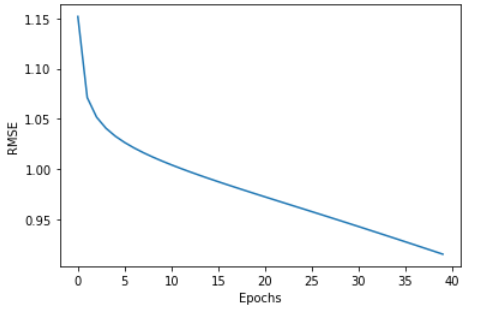
\includegraphics[width=0.5\textwidth]{./200_40_graph.PNG}
	\caption{RMSE graph for rank =200 and epochs = 40}
\end{figure}

50,40
Epoch 39, mse = 0.9447392710872188
Test RMSE: 1.0427012386780807

\begin{figure}[h]
	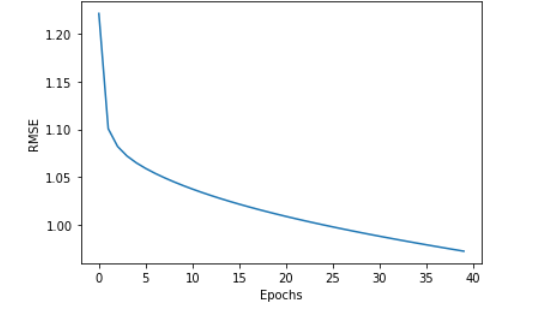
\includegraphics[width=0.5\textwidth]{./50_40_graph.PNG}
	\caption{RMSE graph for rank = 50 and epochs = 40}
\end{figure}

100,60
Epoch 59, mse = 0.9101701523855344
Test RMSE: 1.188729648171058

\begin{figure}[h]
	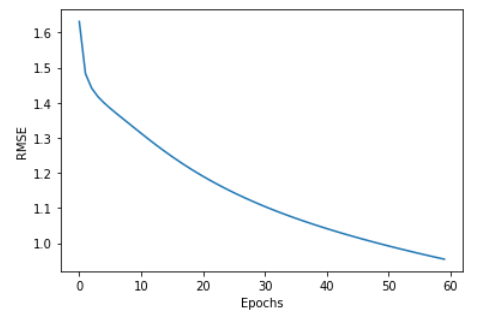
\includegraphics[width=0.5\textwidth]{./100_60_graph.PNG}
	\caption{RMSE graph for rank = 100 and epochs = 60}
\end{figure}

%%%%%%%%%%%%%%%%%%%%%%%%%%%%%%%
% Reference:
% learning rate| regularization (\lamba)| Rank of factorization (k)|Number of epoch (x)| Batch size (N)
% $\lambda$ & $k$ &  $\lambda$ & Train RMSE & Test RMSE
%%%%%%%%%%%%%%%%%%%%%%%%%%%%%%%
% \begin{tabular}{| c | c | c | c | c | c |}
%     \hline
% 	$\lambda$ & $k$ &  $x$ & $N$ & Train RMSE & Test RMSE\\
%     \hline
% 		$100$ & $0.005$ & $0$ & $0$ & $0.41625$ & $1.26925$ \\
%     \hline
% 		$100$ & $0.005$ & $0.01$ & $0$ & $0.40730$ & $1.15628$ \\
%     \hline
% 		$50$ & $0.005$ & $0$ & $0$ & $0.54142$ & $1.08247$ \\
%     \hline
% 		$10$ & $0.005$ & $0$ & $0$ & $0.724214$ & $0.954739$ \\
%     \hline
% 		$100$ & $0.01$ & $0$ & $0$ & $0.27$ & $1.37$ \\
%     \hline
% \end{tabular}\\

\hspace{2em}

% \begin{tabular}{| c | c | c |}
%     \hline
%     \multicolumn{3}{|c|}{\textbf{Spearman}}\\
%     \hline
%     $k$ & Aggregation function & RMSE\\
%     \hline
%     $10$ & Naive arithmetic mean & $1.2084831045336266$\\
%     \hline
%     $10$ & Weighted & $1.208482338367309$\\
%     \hline
% \end{tabular}

\hspace{10em}

% The significantly higher RMSE is most likely because of lack of cooresponding data for the movie due to a truncated dataset.
% It is expected that the test RMSE shall increase significantly as we switch to a larger training dataset in the future.

% It is also worth noting from models 3 and 4 that,
% although the training RMSE is much higher than the previous models,
% they have much lower test RMSE than the others.
% In particular, the fourth model is the first one to achieve test RMSE below $1$.
% It is hence concluded that reducing rank is very helpful in preventing overfitting the model.
% This is also reasonably justified by the fact that
% matrix factorization is otherwise just a meaningless copy of the original matrix
% if the reduced rank is comparable to the original size ($10/50/100$ vs $1000$ vs $10000$ in this case).

% In contrast, setting a higher learning rate $\alpha = 0.01$ as in model 5
% has achieved the lowest train RMSE of all models,
% but also the highest test RMSE.
% This reflects that the SVD model is very vulnerable to overfitting.

% \begin{figure}
% 	\caption{RMSE plot for the first model}
% 	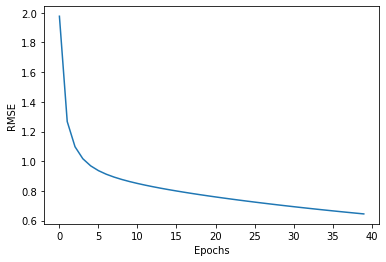
\includegraphics[width=0.5\textwidth]{./svd1.png}
% \end{figure}


% \subsection{Further enhancement}
% We plan to split the bias terms $b_u$ and $c_i$ into terms binned by weekday or day-of-year,
% i.e. $b_{u,t}, c_{i,t}$.
% This allows the model to take into account effects of time on user ratings.
% BigChaos~\cite{BigChaos2008} noted that this approach is helpful in offsetting long-term (probably emotional) drift of the user over time.

{\small
	\bibliographystyle{ieee_fullname}
	\bibliography{egbib}
}

\end{document}
